% do not change these two lines (this is a hard requirement
% there is one exception: you might replace oneside by twoside in case you deliver 
% the printed version in the accordant format
\documentclass[11pt,titlepage,oneside,openany]{article}
\usepackage{times}


\usepackage{graphicx}
\usepackage{latexsym}
\usepackage{amsmath}
\usepackage{amssymb}
\usepackage[utf8]{inputenc}
\usepackage{ntheorem}

% \usepackage{paralist}
\usepackage{tabularx}

% this packaes are useful for nice algorithms
\usepackage{algorithm}
\usepackage{algorithmic}

% well, when your work is concerned with definitions, proposition and so on, we suggest this
% feel free to add Corrolary, Theorem or whatever you need
\newtheorem{definition}{Definition}
\newtheorem{proposition}{Proposition}


% its always useful to have some shortcuts (some are specific for algorithms
% if you do not like your formating you can change it here (instead of scanning through the whole text)
\renewcommand{\algorithmiccomment}[1]{\ensuremath{\rhd} \textit{#1}}
\def\MYCALL#1#2{{\small\textsc{#1}}(\textup{#2})}
\def\MYSET#1{\scshape{#1}}
\def\MYAND{\textbf{ and }}
\def\MYOR{\textbf{ or }}
\def\MYNOT{\textbf{ not }}
\def\MYTHROW{\textbf{ throw }}
\def\MYBREAK{\textbf{break }}
\def\MYEXCEPT#1{\scshape{#1}}
\def\MYTO{\textbf{ to }}
\def\MYNIL{\textsc{Nil}}
\def\MYUNKNOWN{ unknown }
% simple stuff (not all of this is used in this examples thesis
\def\INT{{\mathcal I}} % interpretation
\def\ONT{{\mathcal O}} % ontology
\def\SEM{{\mathcal S}} % alignment semantic
\def\ALI{{\mathcal A}} % alignment
\def\USE{{\mathcal U}} % set of unsatisfiable entities
\def\CON{{\mathcal C}} % conflict set
\def\DIA{\Delta} % diagnosis
% mups and mips
\def\MUP{{\mathcal M}} % ontology
\def\MIP{{\mathcal M}} % ontology
% distributed and local entities
\newcommand{\cc}[2]{\mathit{#1}\hspace{-1pt} \# \hspace{-1pt} \mathit{#2}}
\newcommand{\cx}[1]{\mathit{#1}}
% complex stuff
\def\MER#1#2#3#4{#1 \cup_{#3}^{#2} #4} % merged ontology
\def\MUPALL#1#2#3#4#5{\textit{MUPS}_{#1}\left(#2, #3, #4, #5\right)} % the set of all mups for some concept
\def\MIPALL#1#2{\textit{MIPS}_{#1}\left(#2\right)} % the set of all mips





\begin{document}

\pagenumbering{roman}
% lets go for the title page, something like this should be okay
\begin{titlepage}
	\vspace*{2cm}
  \begin{center}
   {\Large Information Retrieval Project Report \\}
   \vspace{2cm} 
   {Class Project\\}
   \vspace{2cm}
   {presented by\\
    Michael Dell (1359433), Alexander Müller (1376818), Maxim (1237121)  \\
    
   }
   \vspace{1cm} 
   {
    University of Mannheim\\} \vspace{2cm}
   {July 2014}
  \end{center}
\end{titlepage} 

% no lets make some add some table of contents
%\tableofcontents
\newpage

%\listofalgorithms

%\listoffigures

%\listoftables

% evntuelly you might add something like this
% \listtheorems{definition}
% \listtheorems{proposition}

\newpage


% okay, start new numbering ... here is where it really starts
\pagenumbering{arabic}
\section{Introduction and Problem Statement}
Finding information on the web has, thanks to Google, became a lot easier over the years. New algorithms and technologies have made this task more convenient and the precision with which search engines retrieve information is astounding.

One of the most important and prevalent search queries nowadays are people lookups, e.g. finding information on a person like their biography and contact information. In the past, if you wanted to find someone’s address or phone number you would look it up in a phone book. Today, a simple query on Google gets you that information in seconds (for celebrities and other important people at least).

However, extracting the right information from the vast amount of unstructured documents and web pages on the internet is not a trivial task. A lot of research is going into improving extraction algorithms such as Named Entity Recognition and Natural Language Processing algorithms.

The University of Mannheim has a large online presence with thousands of web pages that contain all sorts of information including personal information on university staff. This project introduces a web-based search engine that specializes in retrieving contact information from the university’s domain. The big challenge is the extraction of this information from a highly unstructured data set of several hundred thousand web pages. Additionally, there is no common representation for this contact data between the different chairs of the university which makes this task even more problematic.

The most obvious use of our search engine is finding university staff by their name, however this is not the only way the engine can be utilized. There is also the possibility of a field search that is useful whenever you have information like an email address or a phone number and you want to find out who they belong to.



\section{Architecture Overview}
The figure \ref{fig:overview} below shows the main components of our system. The left part is dedicated to the data gathering, extraction and storing, whereas the right part displays the indexing and actual searching capabilities. All steps will be described in detail in the following chapter.

\begin{figure}[htb]
  \begin{center}
   
\includegraphics[width=1.0\textwidth]{figures/overview.png}
  \end{center}
  \caption{The user interface}
    \label{fig:overview}
\end{figure}


\section{Components}

\subsection{Crawler}
Since we are relying only on information encoded in standard, publicly available web pages we use a well known crawler, namely Apache Nutch\footnote{http://nutch.apache.org/} in order to discover and store links to all websites. The crawler has been configured such, that the crawl is limited to sites hosted within the uni-mannheim.de top level domain and its respective subdomains. In addition we filter all pages which do not contain any or to less HTML code, like hosted PDF files or pure text documents.

\subsection{HTML Parser}
The received HTML documents are fully parsed in order to create a DOM tree representation of the websites structure. We therefore use the popular Java library jsoup\footnote{http://jsoup.org/}. As almost all pages within the uni-mannheim.de-domain are created with the use of content management systems they follow a similar structure. We exploit this fact by ignoring some parts of the sites like headers or navigation links, thus focusing on the actual content of the page which most likely carries most meaningful information. A typical page containing contact details is shown in figure~\ref{fig:contact} In addition to that this approach allows us to keep the information about the actual DOM elements which contain specific data, for example to differentiate if a name appears in a headline or a standard paragraph. For further explanation of the field information extraction see the following section.

\begin{figure}[htb]
  \begin{center}
   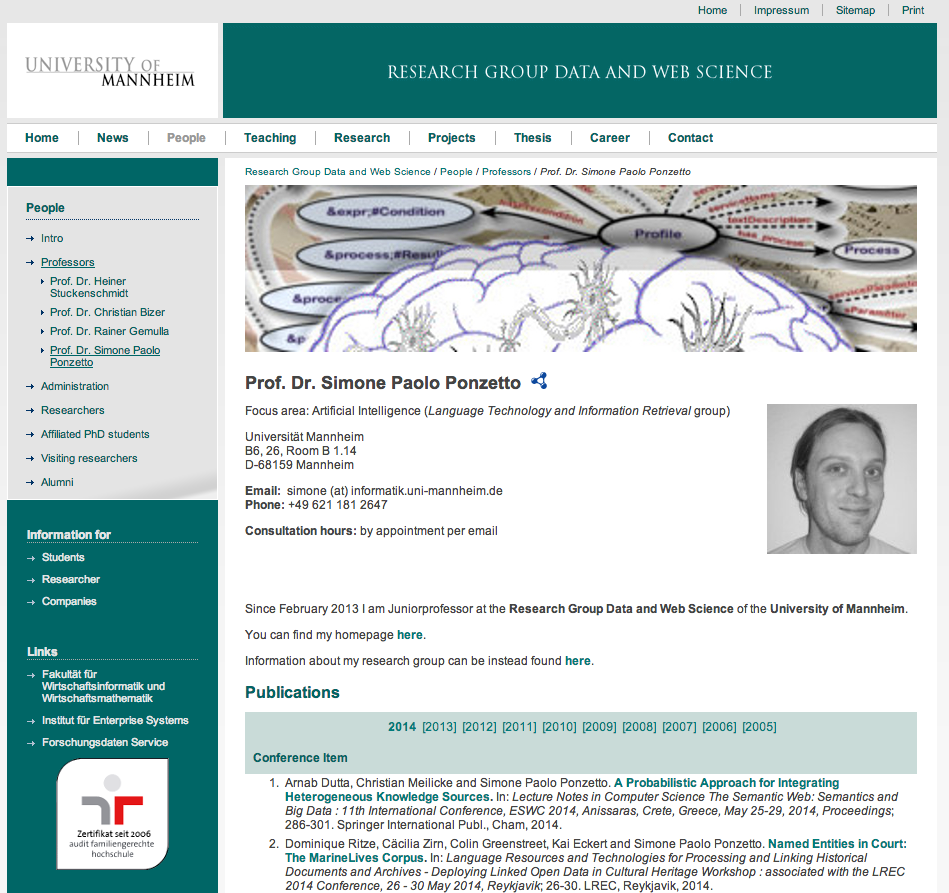
\includegraphics[width=1.0\textwidth]{figures/contact.png}
  \end{center}
  \caption{A typical page containing contact information}
    \label{fig:contact}
\end{figure}


\subsection{Person Contact Information Extraction}

\textbf{General Approach}\\
Since the DOM follows a tree-like structure, but not only leaf nodes can contain useful information we apply a recursive approach. Thereby we focus only on areas of the page where we assume the most meaningful information, specific to that particular site, as described above. We then filter all nodes containing text longer than a specified threshold, if a node contains child nodes only the elements own text is considered and the child nodes are treated recursively. Furthermore, the extracted text is split again on line breaks encoded in HTML. The resulting text fragments are handled by a heuristical parser afterwards, which checks whether the  fragment contains one or more pieces of contact information like a phone number and tries to extract them. Therefore we apply different heuristics for each field. Because of this and due to the fact that one fragment could contain information about more than one field all fragments are handled by all heuristics simultaneously. Two of these heuristics, namely the named entity, that is in our case the full name as well as the titles of a person, and the email address extraction, will be introduced exemplarily. In general all heuristics follow the approach to prefer ‘higher’ nodes over ‘lower’ ones in the DOM tree. This relates to the appearance within the tree, but also to a semantic hierarchy of the elements. For example information found in a h1-tag will be prefered over information contained in h2-tag.\\


\textbf{Example: Email address extraction}\\
For email extraction first, only anchor elements indicating a mail address, i.e. starting with ‘mailto:’ are extracted, since we assume these elements to contain the most accurate information. If this step does not deliver any results, next we will match all pure text elements against a set of regular expression designed to identify and extract proper email addresses, as well as blurred addresses embedded within other text, like ‘person (AT) mail.uni-mannheim.de’. If such cases are extracted, they will be further sanitized in order to store a valid email address, for example by replacing ‘(AT)’ with the ‘@’ character. 

After we exploited the structure of the website, the need of having additional checks whether the heuristic really extracted a person or not came up. Therefore we decided to make use of Name Entity Recognition (NER). NER is defined as the identification of proper names in text or collection of text and assign them to a category person, location and organization. Due to our problem domain we only considered Named Entities (NE) of the type Person. 

A well-known library for Natural Lange Processing (NLP) tasks is Stanford Core NLP \cite{manning2014}, which also includes in their current version a NER Component to recognize English names. Of course this is not optimal and therefore we combined the current version of Stanford Core NLP with an older where a German NER Component exists \cite{faruqui10}. 

In the evaluation Chapter we will investigate how this two different libraries performed. 
Consequently we used for our purposes both NER Components in combination. As illustrated above we exploit the html structure of a webpage. Therefore we iterate over the DOM Structure and only consider header elements. If in one heading, one of the NER Components finds a NE of type Person, the algorithm tries to extract contact information in the corresponding parts of the html documents, otherwise it continues.
The result of this step of our pipeline is a set of person entity candidates that still can contain corrupt or duplicate data. Therefore the next step is to clean the set.


\subsection{Candidate Pruning}
The person entities extracted in the previous step of the extraction pipeline can still contain a lot of corrupt data.  Some examples are extractions that relate to a NE in the heading, but no contact data in the related parts like: “Publications of Prof. Dir. Simone Paolo Ponzetto”. Furthermore there will be a lot of duplicates in the resulting set, because lots of university employees do have their contact data on duplicate webpages.

To solve the first case we once more analyze the heading that lead to the extraction of contact data and count how many of the words are on a name word list. If this is more than one third we consider them this as a correctly extracted Person entity. 
Second to eliminate duplicate entries we developed a light-weight heuristic to identify them. For the ease of use we define that two people are duplicate entities when first name, last name and the email address are the same. Now the question arose which one to keep? For further improving the performance of our system we decided to keep the entity with most not null values in its fields.
After this step the set of candidate entities was pruned in order to assure a high data quality.


\subsection{Enable Search with Apache Solr}

In the previous chapters the extraction of person entities associated with their contact data was presented. In order to make this information accessible to end-users, to fulfill their information need an information retrieval system is necessary. A special requirement is fulfilling the need of field queries for the purpose of inverse searches. For instance if a user got a call from a telephone number he doesn't know, he want to retrieve all people that have the corresponding number.

An ideal system to fulfill those user requirements is Apache Solr, which was developed as all-in-one information retrieval/search engine. It fulfills the tasks of index creation, both for free-text queries and field search, as well as the handling and parsing of user queries.  Since our problem the search problem in our case is not an typical search on unstructured or semi-structured data residing in textual documents we need to change the configuration of Apache Solr.

\begin{figure}
  \begin{center}
   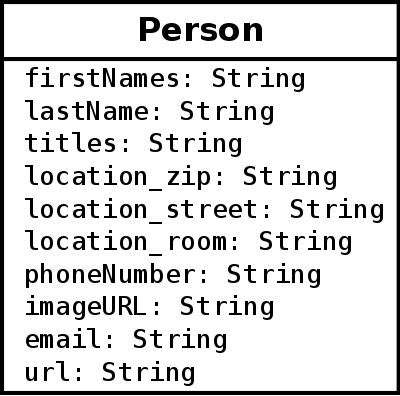
\includegraphics[width=0.38\textwidth]{figures/Person.png}
  \end{center}
  \caption{Datastructure of a Person Entity}
    \label{fig:person}
\end{figure}

The entities that were extracted are stored in a MySQL database with the representation as shown in Figure \ref{fig:person}.  In order to allow Solr to access the database we needed to change some of the configuration parameters. First of all necessary java classed needed to be included to allow Solr to establish a JDBC connection to the database the entities reside in. Now we enabled the creation of inverted indices both, for field queries and free text queries considering all fields when the user enters his or her query. 

This query interface is in Apache Solr by default exposed via webservices, which we used to communicate to our custom build User Interface which will be described in the following section.



\subsection{User Interface}
The basic user interface is shown in figure \ref{fig:ui}. 

\begin{figure}[hbt]
  \begin{center}
   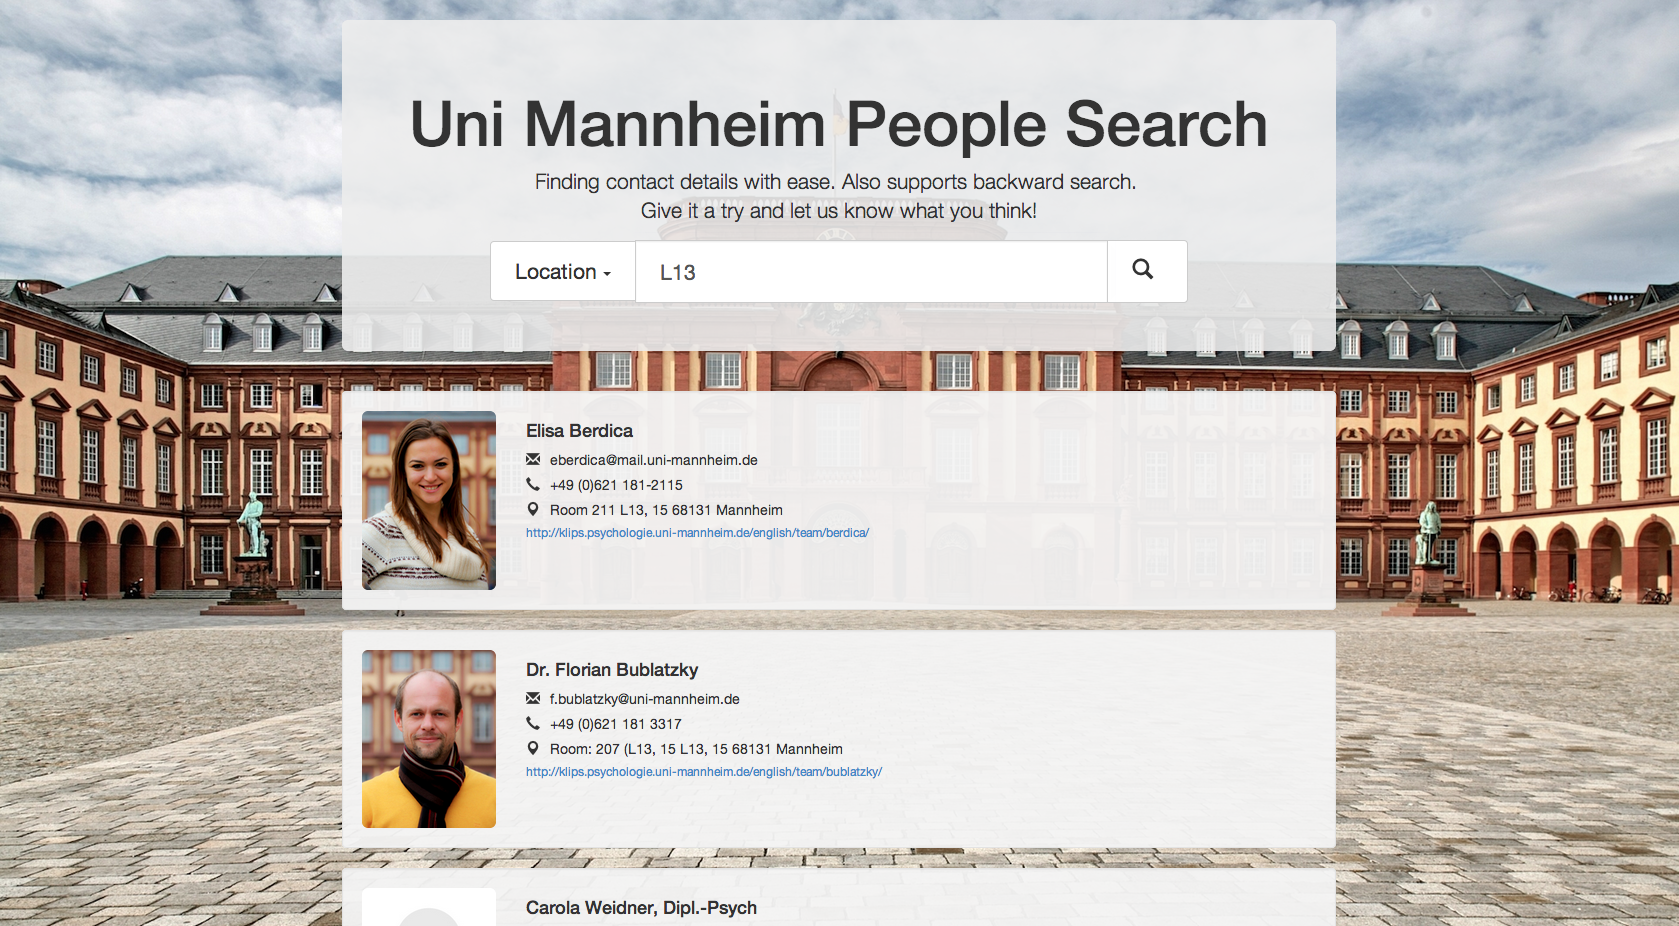
\includegraphics[width=1.0\textwidth]{figures/ui.png}
  \end{center}
  \caption{The user interface}
    \label{fig:ui}
\end{figure}

The user interface is implemented as a modern, single page application which communicates with Solr’s Json interface using Ajax calls, thus trying to optimize the users perceived performance of the system. Initially the page consists of a single input field adjacent to a drop down menu letting the user limit the search to a specific field. If no field is selected all fields will be taken into account. Furthermore the user can use wildcards at any time.
The results will be displayed below in a list view, which simulates the appearance of business cards, as we expect the user to be familiar with this presentation of a person's contact information. The displayed information is very concise and includes a picture, the persons full name and title, email address, telephone number, physical address with room number as well as a link to the original page where these information have been extracted from.

\section{Project Evaluation}
In order to evaluate the precision and recall of the application we first have to look at the amount of entries that have been written into the SQL database. With 1216 entries we have covered a sizable part of the staff considering that there are about 1537 people working at the university.\footnote{http://www.uni-mannheim.de/1/universitaet/profil/zahlen\_geschichte/} If we take into account that some of those do not have a web profile we are actually pretty close to full coverage.

However, since we cannot guarantee that the web crawl with Nutch includes all web pages under the university domain there might be some pages that were not processed by our application leading to possible missing contacts.

By utilising our custom built HTML extractor in combination with a NER engine we can distinguish a real person’s contact information from random useless text pretty accurately. Unfortunately, the precision still is not 100\% so that a few of the extracted people do not actually exist. This, however, is not a problem because those entries should never get retrieved during search anyway.

Another problem we faced while running the extraction are random time-outs while accessing the web pages. Even with a very generous 10 seconds for pages that are not responding as quickly, we still got a sizable amount of web pages that are not reachable and that might contain information that is relevant to our application.

In order to reduce the amount of spam they receive some staff members or chairs try to obscure their email address by intentionally using blank spaces or replacing the @ and/or dots. This, however, also complicates the extraction of these email addresses which is certainly the intention. Our algorithm recognizes email addresses as such pretty accurately. Unfortunately, some staff members encode their email address in a picture which makes a successful extraction within the scope of this project impossible. 


\section{Summary}
In this project we first utilized the web crawler Apache Nutch to index all the web pages belonging to the University of Mannheim domain and its chairs which turned out to be around 500.000 pages. Since we were not interested in documents such as PDFs or Word documents as they do not contain contact information we eliminated those from the start leaving us with just over 490.000 pages that needed processing. We then built a parallelized Java tool that tries to extract relevant information from each of those pages by utilizing different techniques such as NER, regular expressions and common names lists. After processing the web pages with this tool the program automatically loaded the extracted information into an SQL database from which we built an index with Apache Solr.
Solr now allows us to run search queries on that data which is then returned in JSON format. The UI then fits the JSON data into nice info boxes and displays those to the user.



%\bibliographystyle{plain}
%\bibliography{thesis-ref}


%\appendix



\newpage



\bibliographystyle{plain}
\bibliography{thesis-ref}


\end{document}
